\documentclass[a4paper]{article}
\usepackage[left=1cm, right=1cm, top=1cm, bottom=1cm]{geometry}
\usepackage{amsmath}
\usepackage{amssymb}
\usepackage{amsfonts}
\usepackage{subcaption}
\usepackage{caption}
\usepackage{graphicx}
\usepackage{fullpage}
\usepackage{textcomp}
\usepackage{listings}
\usepackage{float}
\usepackage[toc,page]{appendix}

% hyperref must be last
\usepackage{hyperref}
\hypersetup{
  backref=true,
  colorlinks=true,
  linkcolor=blue,
  citecolor=blue,
  urlcolor=blue
}

\title{Shape Optimization of Wind Spar}
\author{ID:4873}
\begin{document}
 \maketitle
 
\begin{abstract}
   In this project we design the shape of a wing spar using numerical optimization techniques such that given total weight of an aircraft and material property, the weight of the spar is minimized. This problem is representative of numerical optimization in that it involves three basic ingredients, the shape parameterization, the PDE (partial differential equation) solver, and the optimization tool. We first describe the analysis method, the geometry parameterization, and the mathematical statement of the design problem, then results and conclusion are given.
\end{abstract}

\section{Physics Model} \label{sec:physics}
The wind spar is used to support the aerodynamic force acting on the aircraft. The cross-section shape of the spar in this project is a circular annulus, with size constraints as follows
\begin{equation}
\begin{aligned}
r &\ge 0.02m \\
R &\le 0.05m \\
R-r &\ge 0.0025m\\
\end{aligned}
\end{equation}
where $r$ and $R$ are the inner and outer radius of the circular annulus, respectively.
The spar is made of carbon fiber composite, with density $1600\:km/m^3$, Young's modulus $70\:GPa$, and ultimate tensile/compressive strength $600\: MPa$.

The loading on the spar is $2.5$ times the weight of the aircraft, and the force is assumed to be linearly distributed, with maximum load at the root and zero load at the tip.

The objective is to minimize the weight of the spar without the structure reaching the ultimate strength of the carbon fiber. 
\section{Mathematical Model}
\subsection{Optimization problem}
To use an numerical optimization technique, the physics model in Section~\ref{sec:physics} must be rewritten into a mathematical model. The one used in this work is as follows:
\begin{equation} \label{eq:math_model_1}
\begin{aligned}
max\:\: &f(r(x), R(x)) \\
s.t.\:\: & r(x) \ge 0.02 \\
         & R(x) \le 0.05 \\
         & R(x)-r(x) \ge 0.0025 \\
         &\sigma(r(x), R(x)) \le \sigma_{yield}
\end{aligned}
\end{equation}
where $\sigma_{yield}$ is ultimate strength of the fiber, $f$, the objective function, is the weight of the spar, 
\begin{equation*}
f = \int \pi (R^2 - r^2) dx
\end{equation*}
and $\sigma$ the stress of the spar subject to the loading. The relation between the stress and the shape of the spar ($r$ and $R$) is governed by the Euler-Bernoulli beam equation:
\begin{equation}\label{pde}
\begin{aligned}
{\cfrac  {\partial ^{2}}{\partial x^{2}}}\left(EI{\cfrac  {\partial ^{2}w}{\partial x^{2}}}\right)=q(x)\\
\sigma =-zE~{\frac  {{\mathrm  {d}}^{2}w}{{\mathrm  {d}}x^{2}}}
\end{aligned}
\end{equation}
where $q$ is the loading force, $E$ the Young's modulus, $I$ the second moment of area, $w$ the the deflection of the spar. In this specific problem, the linearly distributed force $q=500*2.5*9.8/L (1-x/L)$.

See \url{https://en.wikipedia.org/wiki/Euler%E2%80%93Bernoulli_beam_theory} for more infomation on the Euler-Bernoulli beam theory.


\section{Analysis model} \label{sec:analysis_tool}
\subsection{Shape optimization}\label{shape_param}
Although appearing concise, this problem cannot be solved analytically, and numerical methods must be employed. To this end, the inner and outer radius, $r$ and $R$, have to be replaced by some discrete variables, the process of which is called shape parameterization. The shape parameterization used here is a weighted summation of monomials:
\begin{equation}
\begin{aligned}
r(x) &= \sum_{i=1}^{N_{var}/2} a_ix^{i-1}\\
R(x) &= \sum_{i=1}^{N_{var}/2} a_{i+N_{var}/2}x^{i-1}
\end{aligned}
\end{equation}
where $a_i$ is the design variable, and $N_{var}$ is the number of design variables.

There are other alternative choices in the parameterization. For example, we can choose sinusoids with different frequency as basis; we can also use the value of $r$ and $R$ as design variables directly. The reason we choose monomials here is to guarantee the smoothness of the cross-section of the spar, which is a prerequisite of effective of Euler-Bernoulli beam theory.
\subsection{Finite element solver}
In order to compute the stress appearing in the inequality constraints in \eqref{eq:math_model_1}, we need to solve the differential equation \ref{pde}. In this project, the Euler-Bernoulli equation \eqref{pde} is solved with finite element methods.


\section{Implementation}
The implementation in Matlab is attached in Appendix~\ref{app:calcweight}$\sim$\ref{app:run}. 
Since the optimization tool and the analysis function are both available, the main task is to give the shape parameterization, objective, linear and nonlinear constraints, as well as their gradients with respect to the design variables. Once this variables and functions are defined, we then build the workflow of the optimization process. In order to fit in this workflow, we have to define some wrapper function according the the API of \texttt{fmincon}:
\subsection{Objective function and its gradient}\label{sec:obj}
In this project, we feed in \texttt{fmincon} the objective function and its gradient through a single function. This function should only take design variable as inputs, with signature being:

  \hspace{10 mm}\texttt{function [obj, dobj\_da] = obj\_func(a)}\\
This function is realized in two steps:
\begin{itemize}
  \item first, we define a function
  
  \hspace{10 mm}\texttt{function [obj, dobj\_da] = objFunc(x,a)}\\
  inside which \texttt{calcWeight} and \texttt{calcWeightDerivative} are called to return the objective value $f$ and its gradient $\frac{df}{da}$. See Appendix~\ref{app:calcweight} and \ref{app:calcweightderiv} for the definition of these two functions.
  \item then, an anonymous function is defined within the scope of \texttt{x} to meet the API of \texttt{fmincon}:
  
  \hspace{10 mm}\texttt{obj\_func = @(a) objFunc(x, a)}
  
\end{itemize}

\subsection{Nonlinear constraints}
In Appendix~\ref{app:noncon} and \ref{app:nonconderiv}, the nonlinear constraint and its derivative with respect to the design variables are defined. There are three main steps in \texttt{calcStressConstraints}:
\begin{itemize}
  \item call function \texttt{CalcBeamDisplacement} to get the displacement $u$;
  \item call function \texttt{CalcBeamStress} to get the stress at each node;
  \item build the constraint $c_{ineq} = \frac{\sigma}{\sigma_{yield}}-1$. We use this expression instead of $c_{ineq} = \sigma - \sigma_{yield}$ to reduce the magnitude of the constraints from $O(10^6)$ to $1$. 
\end{itemize}
As for \texttt{caclIneqDerivative}, we use complex-variable methods to compute the the gradient of nonlinear constraints with respect to the design variable.  

As see, both functions have the signature which does not meet the API requirement of \texttt{fmincon}. The same trick in Section~\ref{sec:obj} is played again to address this problem. 

\subsection{Geometric constraints}
Since \texttt{fmincon} only accepts linear constrains in the form of $Ax \le b$, the geometric constraints in \eqref{eq:math_model_1} must be transformed into this form. As mentioned in \ref{shape_param}, we use monomials as the basis of shape optimization. Then the structure of the linear geometric constraints looks like 
\begin{equation*}
\begin{bmatrix}
-A & 0 \\ 0 & A \\ A & -A
\end{bmatrix} a \le \begin{bmatrix}
-0.02 \\ 0.05 \\ 0.0025
\end{bmatrix}
\end{equation*}
where submatrix $A$ is the Vandermonde matrix with dimension \texttt{size(x,1) $\times$ size(a,1)}.

Note, in the code we multiply the geometric constraints with a factor of $100$ to increase the value to $O(1)$ in order to match the nonlinear constraints in magnitude. Otherwise, the optimizer would focus extensively on the nonlinear constraints rather than the geometric constraints, and yield invalid shape with $R\le r$ which definitely fail the finite element solver.

The geometric constraints are realized in Appendix~\ref{app:getgeomcon}.

\section{Results and discussion}
12 cases were run to study the performance of current method, with the order of monomial basis from $1\sim 4$, and 3 different grids. In all cases the same initial shape is specified which corresponds to linear $r=0.04635$ and $R=0.05$ with $f_{init} = 1.325793e+01$. 

Table~\ref{tb:weight} lists the weight of the spar while Figure.~\ref{fig:final_shape} show the inner and outer shape of the circular annulus. $46.29\% \sim 62.28\%$ reduction in weight is achieved after the design.

As can be seen in Table~\ref{tb:weight}, with the same basis in shape parameterization, the weight of the spar does not change very much as the number of elements is increased. However, from Figure.~\ref{fig:final_shape} we can see the final shapes are significantly different from grid to grid, especially when order is larger than 2.

On the other hand, the results heavily depend on the order of the basis. Specifically, the higher the order of the basis, the smaller the optimized weight.
\begin{table}[h]
  \begin{center}
    \caption[]{Optmized weight of spar} \label{tb:weight}
     \begin{tabular}{p{0.05\textwidth}p{0.15\textwidth}p{0.15\textwidth}p{0.15\textwidth}}
       \hline
       order&      nElems=5  & nElems=10   & nElems=20 \\
        \hline
        1&          7.087691e+00 &  7.112617e+00 &   7.120396e+00  \\
        2&          5.664373e+00 &  5.719084e+00&    5.755517e+00 \\
        3&          5.175438e+00&   5.222951e+00&     5.241904e+00    \\
        4&          5.000245e+00&   5.037060e+00&     5.066670e+00\\
        \hline
     \end{tabular}
  \end{center}
\end{table}


\begin{figure} [H]
  \begin{subfigure}{0.51\textwidth}
    \centering
    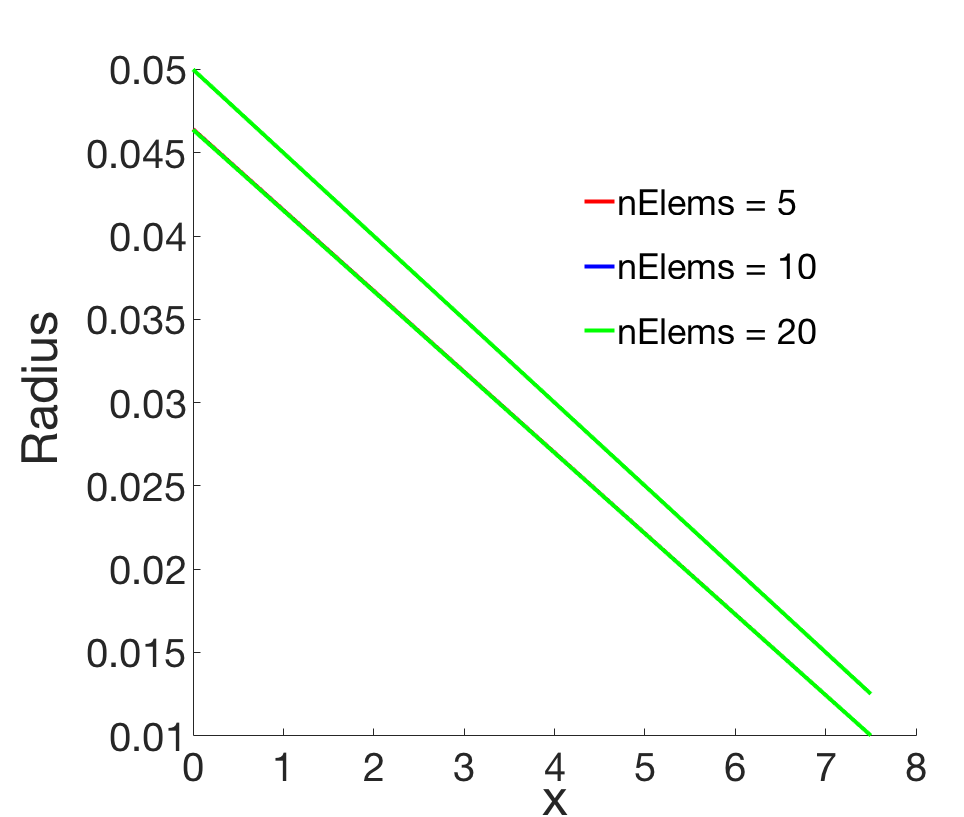
\includegraphics[width=1.0\linewidth]{p1.png}
    \subcaption{linear}
    \label{fig:linear}
  \end{subfigure}
  \begin{subfigure}{0.51\textwidth}
    \centering
    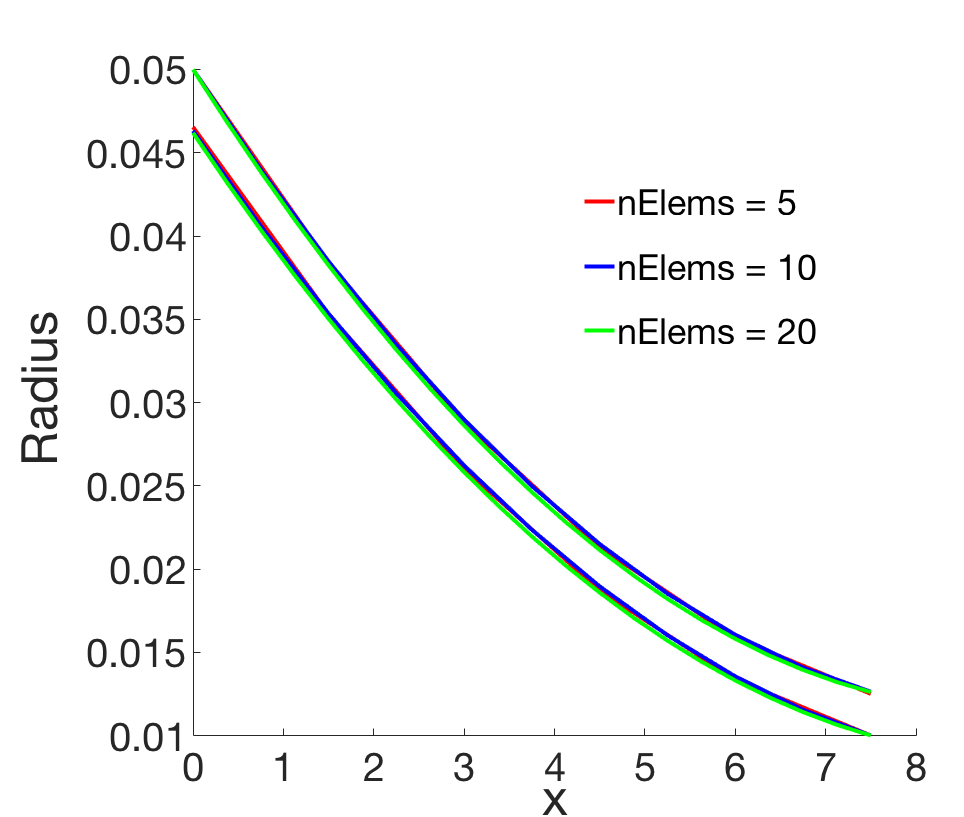
\includegraphics[width=1.0\linewidth]{p2.png}
    \subcaption{quadratic}
    \label{fig:quadratic}
  \end{subfigure}\\[4ex]
  \begin{subfigure}{0.51\textwidth}
    \centering
    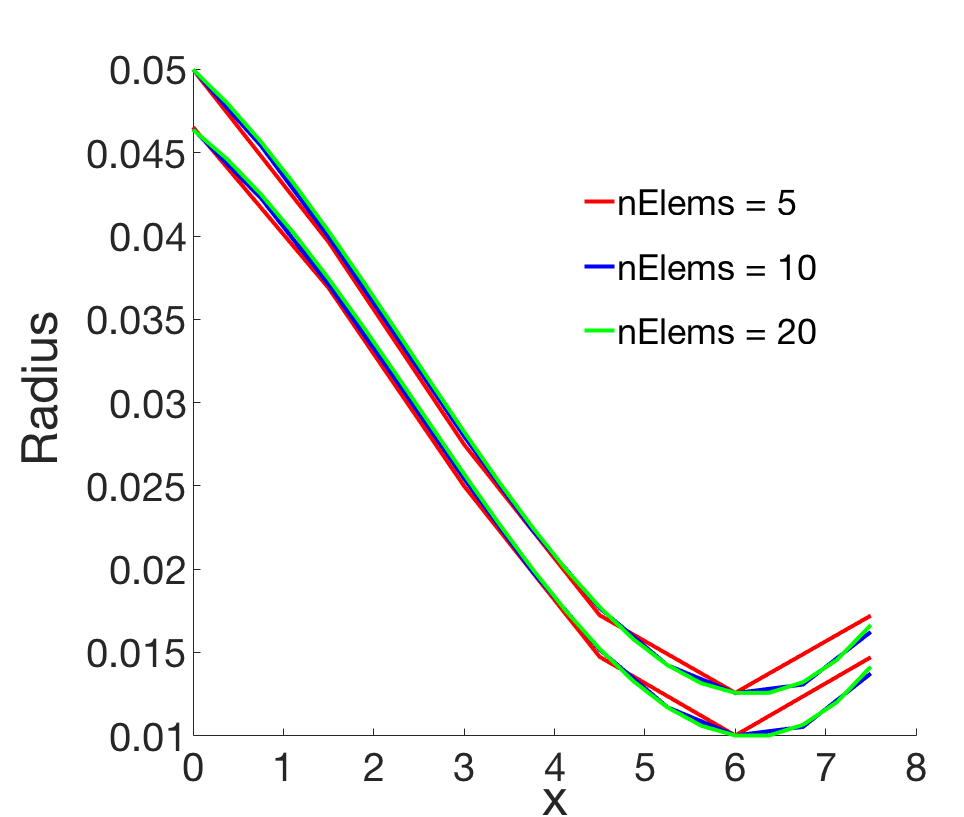
\includegraphics[width=1.0\linewidth]{p3.png}
    \subcaption{cubic}
    \label{fig:cubic}
  \end{subfigure}
  \begin{subfigure}{0.51\textwidth}
    \centering
    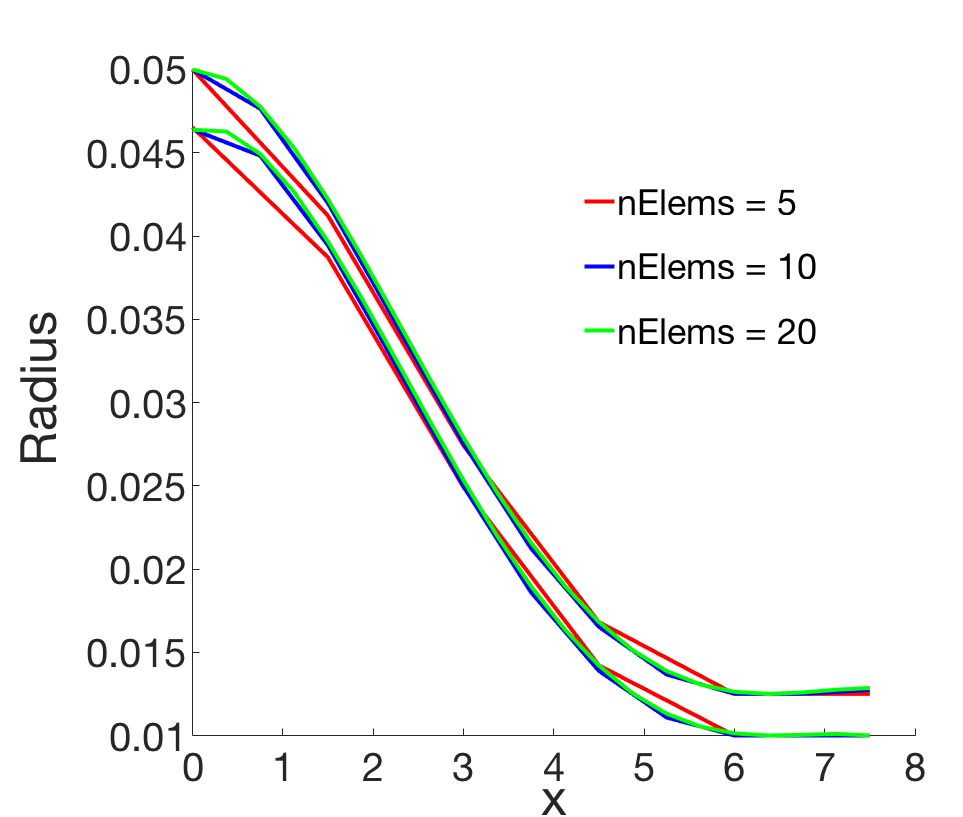
\includegraphics[width=1.0\linewidth]{p4.png}
    \subcaption{quartic}
    \label{fig:quatic}
  \end{subfigure}  
  \caption{Optimized shape of circular annulus  \label{fig:final_shape}}
\end{figure}

\section{Conclusion}
In this work, we use numerical optimization design technique to reduce the weight of a wing spar. The spar is parameterized with monomial basis to guarantee the smoothness of the cross-section, which is needed by the Euler-Bernoulli beam theory. Complex-variable methods are used to compute the derivative of objective and nonlinear constraints. The results see significant reduction in spar weight, which proves the effective the current methods.

\small
\begin{appendices} 
\section{calcWeight.m}\label{app:calcweight}
\begin{lstlisting}[language=Matlab]
function [ weight ] = calcWeight( x, a )
%
% Calculate the weight of spar
%
density = 1600;
nElems = size(x, 1) - 1;
% get inner and outer radii
[r, R] = geomParameterization(x, a);
% loop over all elements, accumulate the volume
weight = 0.0;
for i = 1 : nElems
  dx = x(i+1) - x(i);
  area = R(i+1)*R(i+1) - r(i+1)*r(i+1) + R(i)*R(i) - r(i)*r(i);
  weight = weight + area * dx;
end
% factor pi comes from S = pi*R^2; 
% factor 0.5 comes from average of bottom and top area of each element.
weight = weight * 0.5 * pi * density;
end

\end{lstlisting}

\section{calcWeightDerivative.m}\label{app:calcweightderiv}
\begin{lstlisting}[language=Matlab]
function [ dwda ] = calcWeightDerivative( x, a )
%
% complex-variable method to compute the gradient of weight
% w.r.t the design variable.
%
nVars = size(a, 1);
dwda = zeros(nVars, 1);
eps = 1.0e-12;
for i = 1 : nVars
  a(i) = a(i) + complex(0.0, eps);
  weight = calcWeight(x, a);
  dwda(i) = imag(weight) / eps;
  a(i) = a(i) - complex(0.0, eps);
end
end

\end{lstlisting}

\section{objFunc.m}\label{app:calcobj}
\begin{lstlisting}[language=Matlab]
function [ obj, dobj_da ] = objFunc( x, a )
%
% this function is wrapper of objective function
% and its gradient
%
obj = calcWeight(x, a);
if nargout > 1 
  dobj_da = calcWeightDerivative(x, a);
end
end
\end{lstlisting}

\section{caclStressConstraints.m}\label{app:noncon}
\begin{lstlisting}[language=Matlab]
function [ cineq, ceq ] = calcStressConstraints( L, E, force, x, a )
%
% This function is a wrapper for the nonlinear constraints.
%
nx = size(x, 1);
nElems = nx - 1;
% get inner and outer radii
[r, R] = geomParameterization(x, a);
% compute 2nd moment of area
Iyy = 0.25*pi * (R.^4 - r.^4);
if min(R-r) <= 0.00
error("the outer radius is smaller than the inner")
end
% compute displacements (vertical and angle)
u = CalcBeamDisplacement(L, E, Iyy, force, nElems);
% compute stess
cineq = CalcBeamStress(L, E, R, u, nElems);
sigma_yield = 600.0e6;
cineq = cineq / sigma_yield - 1;
ceq = [];
end
\end{lstlisting}

\section{calcIneqDerivative.m}\label{app:nonconderiv}
\begin{lstlisting}[language=Matlab]
function [ dcineq_da, dceq_da ] = calcIneqDerivative( L, E, force, x, a )
%
% complex-variable method to compute the derivative of inequality
% function w.r.t. design variable a
%
[cineq, ceq] = calcStressConstraints(L, E, force, x, a);
nVars = size(a, 1);
nineq = size(cineq, 1);
neq   = size(ceq, 1);
dcineq_da = zeros(nVars, nineq);
dceq_da   = zeros(nVars, neq);
eps = 1.0e-12;

for i = 1 : nVars
  a(i) = a(i) + complex(0.0, eps);
  [cineq, ceq] = calcStressConstraints(L, E, force, x, a);
  a(i) = a(i) - complex(0.0, eps);
  for j = 1 : nineq
    dcineq_da(i, j) = imag(cineq(j)) / eps;
  end
  for j = 1 : neq
    dceq_da(i, j) = imag(ceq(j)) / eps;
  end
end
end
\end{lstlisting}

\section{calcStressConstraints.m}\label{app:nonlcon}
\begin{lstlisting}[language=Matlab]
function [ cineq, ceq, dcineq_da, dceq_da ] ...
    = calcIneqConstraints( L, E, force, x, a )
[cineq, ceq] = calcStressConstraints(L, E, force, x, a);
if nargout > 2
  [dcineq_da, dceq_da] = calcIneqDerivative(L, E, force, x, a);
end
end
\end{lstlisting}

\section{geomParameterizatio.m}
\begin{lstlisting}[language=Matlab]
function [ r, R ] = geomParameterization( x, a )
%
% This function implements the geometric parameterization.
% Currently, a polynomial is used as basis, that is,
%   r = \sum a_i     x^(i-1)
%   R = \sum a_{i+n} x^{i-1}
%
nhalf = size(a, 1) / 2;
nx = size(x, 1);
r = zeros(nx, 1);
R = zeros(nx, 1);

for i = 1 : nx
  for p = 1 : nhalf
    r(i) = r(i) + a(p)         * x(i)^(p-1);
    R(i) = R(i) + a(nhalf + p) * x(i)^(p-1);
  end
end
end
\end{lstlisting}

\section{getGeomConstraints.m}\label{app:getgeomcon}
\begin{lstlisting}[language=Matlab]
function [ Aineq, bineq ] = getGeomConstraints( x, a )
%
% This function returns the geometric(linear) inequality constrains:
%   -r     <= -0.01
%        R <=  0.05
%    r - R <= -0.0025
% the structure of which looks like this
%
%   | -A  0 |        | -0.01   |
%   |  0  A | |a| <= |  0.05   |
%   |  A -A |        | -0.0025 |
%
% where A is a Vandermonde matrix since we use
% polynomial to parameterize the shape.
%
nVars = size(a, 1);
nhalf = nVars/2;
nx    = size(x, 1);
Aineq = zeros(3*nx, nVars);
bineq = zeros(3*nx, 1);  
subA  = zeros(nx, nhalf);

for i = 1 : nx
  subA(i,1) = 1.0;
  for j = 2 : nhalf
    subA(i, j) = subA(i, j-1) * x(i);
  end
end

Aineq(     1 :   nx,       1 : nhalf) = -subA;
Aineq(  nx+1 : 2*nx, nhalf+1 : nVars) =  subA;
Aineq(2*nx+1 : 3*nx,       1 : nhalf) =  subA;
Aineq(2*nx+1 : 3*nx, nhalf+1 : nVars) = -subA;

bineq(     1 :   nx) = -0.01;
bineq(  nx+1 : 2*nx) =  0.05;
bineq(2*nx+1 : 3*nx) = -0.0025;
% 
% We magnify the linear constraints so that the magnitude is
% on the same order as the nonlinear constraints. Without this
% magnification, the optimimizer may focus exclusively on the 
% nonlinear constraint first/more, and it's easy to get R < r, 
% which would fail the finite element solver.
%
Aineq = Aineq * 1e2;
bineq = bineq * 1e2;
end
\end{lstlisting}

\section{doOptimization.m}
\begin{lstlisting}[language=Matlab]
function [a, x] = doOptimization(nElems, nVars)
L = 7.5;
E = 70e9;
% a linear initial design variable
a0 = zeros(nVars, 1);
a0(1) = 0.04635;
a0(2) = 0.0;
a0(nVars/2+1) = 0.05;
a0(nVars/2+2) = 0.0;
% grid
x = zeros(nElems+1, 1);
for i = 1 : nElems + 1
  x(i) = (i-1) * L / nElems;
end
% linearly distributed force
force = 500*2.5*9.8/L * (1 - x/L);
% get geometric constraints 
[Aineq, bineq] = getGeomConstraints(x, a0);
% objective function
obj_func = @(a) objFunc(x,a);
% nonlinear constraint function
nonlcon = @(a) calcIneqConstraints(L, E, force, x, a);
% parameters of optimizer
options = optimoptions('fmincon',...
                       'SpecifyObjectiveGradient',true, ...
                       'SpecifyConstraintGradient',true, ...
                       'Display','iter', ...
                       'MaxIter', 150);
problem.options = options;
problem.solver = 'fmincon';
problem.objective = obj_func;
problem.Aineq = Aineq;
problem.bineq = bineq;
problem.nonlcon = nonlcon;
problem.x0 = a0;

a = fmincon(problem);
end
\end{lstlisting} 

\section{run.m}\label{app:run}
\begin{lstlisting}[language=Matlab]
pOrder = 2;
nVars = 2*(pOrder+1);
nElems = 10;
[a, x] = doOptimization(nElems, nVars);
[r, R] = geomParameterization(x, a);
% plot the shape
plot(x, r, 'r--', 'LineWidth',2)
hold on
plot(x, R, 'r', 'LineWidth',2)
nElems = 20;
[a, x] = doOptimization(nElems, nVars);
[r, R] = geomParameterization(x, a);

% plot the shape
plot(x, r, 'k--', 'LineWidth',2)
hold on
plot(x, R, 'k', 'LineWidth',2)

hold off
h = legend('inner radius','','outer radius', 'Location', 'best');
legend('boxoff');
rect = [0.55, 0.55, .25, .25];
set(h, 'Position', rect)
set(gca,'FontSize', 20)
pos = get(gca, 'Position');
pos(1) = 0.2;
pos(2) = 0.1;
pos(3) = 0.75;
set(gca, 'Position', pos)
xl = xlabel('x','FontSize', 25);
yl = ylabel('Radius','FontSize', 25);
set(yl, 'Units', 'Normalized', 'Position', [-0.22, 0.2, 0]);
\end{lstlisting} 
\end{appendices}
\end{document}

